%! alt Part of the parabola y = x squared, with the triangle whose vertices have x-coordinates a = 0, b = 2 and c = 3. Its sides have slopes a + b = 2, a + c = 3 and b + c = 5, which is the sum of the x-coordinates at each pair of ends.
%! after_paragraph 1
%! scale 7/10
% The shared preamble of every Kyuclid figure. pipeline/figures turns these colours into theme-aware paint,
% and refuses any other colour, so draw only with them:
%   figink (lines and labels), figaux (construction lines), figaccent (the object the argument turns on),
%   figtint and figaccenttint (light fills).
\documentclass[border=1.5pt]{standalone}
\usepackage{tkz-euclide}
\definecolor{figink}{RGB}{0,0,0}
\definecolor{figaux}{RGB}{85,85,85}
\definecolor{figaccent}{RGB}{192,57,43}
\definecolor{figtint}{RGB}{221,221,221}
\definecolor{figaccenttint}{RGB}{245,213,208}
% tkz-euclide's defaults draw circles, compasses and marks in 50% grey and fill points with a tint.
\makeatletter
\def\tkz@otherlinecolor{figink}
\def\tkz@euc@circlecolor{figink}
\def\tkz@euc@compasscolor{figink}
\def\tkz@euc@mkcolor{figink}
\def\tkz@mk@fill{figink}
\def\tkz@euc@pointfillcolor{figink}
\makeatother
\tkzSetUpLine[color=figink,line width=.7pt]
\tkzSetUpArc[color=figink,line width=.7pt]
\tkzSetUpCompass[color=figink,line width=.5pt]
\tkzSetUpPoint[color=figink,fill=figink,size=3.1pt]
\tikzset{
  every picture/.style={line cap=round,line join=round,color=figink},
  circle style/.append style={color=figink,line width=.7pt},
  aux/.style={color=figaux,line width=.45pt,dash pattern=on 2.6pt off 2pt},
  key/.style={color=figaccent,line width=1pt},
  mk/.style={color=figink,line width=.5pt},
  lbl/.style={color=figink,inner sep=2.2pt},
  len/.style={color=figink,inner sep=1.5pt,font=\small},
}

\begin{document}
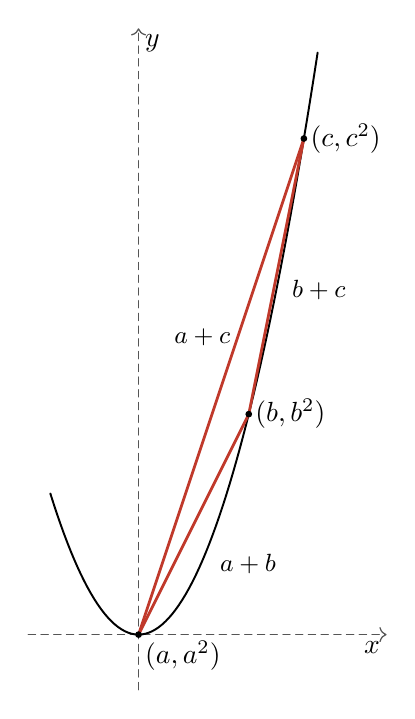
\begin{tikzpicture}
\tkzDefPoint(0.0,0.0){A} %! A = (0, 0)
\tkzDefPoint(1.4000000,2.8000000){B} %! B = (2, 4)
\tkzDefPoint(2.1000000,6.3000000){C} %! C = (3, 9)
\tkzDefPoint(-1.4000000,0.0){XL} %! XL = (-2, 0)
\tkzDefPoint(3.1500000,0.0){XR} %! XR = (4.5, 0)
\tkzDefPoint(0.0,-0.70000000){YL} %! YL = (0, -1)
\tkzDefPoint(0.0,7.7000000){YH} %! YH = (0, 11)
%! fact equal(y(A), x(A)**2)
%! fact equal(y(B), x(B)**2)
%! fact equal(y(C), x(C)**2)
%! fact (y(B) - y(A))/(x(B) - x(A)) == 2
%! fact (y(C) - y(A))/(x(C) - x(A)) == 3
%! fact (y(C) - y(B))/(x(C) - x(B)) == 5
\draw[aux,->] (XL) -- (XR);
\draw[aux,->] (YL) -- (YH);
\draw[line width=.7pt,domain=-1.6:3.25,samples=80] plot ({.7*\x},{.7*\x*\x});
\tkzDrawSegments[key](A,B A,C B,C)
\tkzDrawPoints(A,B,C)
\tkzLabelPoint[below right,lbl](A){$(a,a^2)$}
\tkzLabelPoint[right,lbl](B){$(b,b^2)$}
\tkzLabelPoint[right,lbl](C){$(c,c^2)$}
\tkzLabelSegment[right=15pt,pos=.32,len](A,B){$a+b$}
\tkzLabelSegment[left=1pt,pos=.6,len](A,C){$a+c$}
\tkzLabelSegment[right=5pt,pos=.45,len](B,C){$b+c$}
\tkzLabelPoint[below left,lbl](XR){$x$}
\tkzLabelPoint[below right,lbl](YH){$y$}
\end{tikzpicture}
\end{document}
